
%%%%%%%%%%%%%%%%%%%%%%%%
%%%%%%%%%%%%%%%%%%%%%%%%
%%%%%%%%%%%%%%%%%%%%%%%%
%%%%%%%%%%%%%%%%%%%%%%%%
%%%         V     I     R     T     U     A     L          %%%
%%%%%%%%%%%%%%%%%%%%%%%%
%%%%%%%%%%%%%%%%%%%%%%%%
%%%%%%%%%%%%%%%%%%%%%%%%
%%%%%%%%%%%%%%%%%%%%%%%%
%%%%%%%%%%%%%%%%%%%%%%%%


\section{Adaptive Resampling with Active Learning}
\label{virtual}
The analysis in Section \ref{lotb_experiments} shows the effectiveness of active learning on imbalanced datasets \josh{seems like one kind of model was used?} \seyda{Addressed} without employing any resampling techniques. This section extends the discussion on the effectiveness of active learning for imbalanced data classification, and demonstrates that even in cases where resampling is the preferred approach, active learning can still be used to significantly improve the classification performance.

In supervised learning, a common strategy to overcome the rarity problem is to resample the original dataset to decrease the overall level of class imbalance. Resampling is done either by oversampling the minority (positive) class and/or undersampling the majority (negative) class until the classes are approximately equally represented \cite{Chawla_2002,Japkowicz_2000,Kubat_1997,Ling_1998}. Oversampling, in its simplest form, achieves a more balanced class distribution either by duplicating minority class instances, or introducing new synthetic instances that belong to the minority class \cite{Chawla_2002}. No information is lost in oversampling since all original instances of the minority and the majority classes are retained in the oversampled dataset. The other strategy to reduce the class imbalance is under-sampling, which eliminates some majority class instances mostly by random sampling.

Even though both approaches address the class imbalance problem, they also suffer some drawbacks. The under-sampling strategy can potentially sacrifice the prediction performance of the model, since it is possible to discard informative instances that the learner might benefit.  Oversampling strategy, on the other hand, can be computationally overwhelming in cases with large training sets--- if a complex oversampling method is used,  a large computational effort must be expended during preprocessing of the data. Worse, oversampling causes longer training time during the learning process due to the increased number of training instances. In addition to suffering from increased runtime due to added computational complexity, it also necessitates an increased memory footprint due to the extra storage requirements of artificial instances.\josh{in the past, i've avoided this by using upon request data generation and a small cache.}\seyda{yes, there are tricks to make the challenges manageable, but there may also be application domains where on-demand instance generation and/or caching may not be applicable/feasible. I don't think it's necessary to divert the flow of this section by addressing ways to improve resource utilization.} Other costs associated with the learning process (i.e., extended kernel matrix in kernel classification algorithms) further increase the burden  of oversampling.

\subsection{\textsc{VIRTUAL}: Virtual Instance Resampling Technique Using Active Learning}

In this section, the focus  is on the oversampling strategy for imbalanced data classification and investigate how it can benefit from the principles of active learning. Our goal is to remedy the efficiency drawbacks of oversampling in imbalanced data classification and use an active learning strategy to generate minority class instances only if they can be useful to the learner. \textsc{Virtual} (Virtual Instance Resampling Technique Using Active Learning)~\cite{Ertekin_dissertation} is a hybrid method of oversampling and active learning that forms an adaptive technique for resampling of the minority class instances. In contrast to traditional oversampling techniques that act as an \textit{offline} step that generate virtual instances of the minority class prior to the training process, \textsc{Virtual} leverages the power of active learning to intelligently and adaptively oversample the data \textit{during} training, removing the need for an offline and separate preprocessing stage. Similar to the discussions in the previous section, \textsc{Virtual} also employs an online SVM-based active learning strategy. In this setting, the informativeness of instances are measured by their distance to their hyperplane, and the most informative instances are selected as the support vectors. \textsc{Virtual} targets the set of support vectors during training, and resamples new instances based on this set. Since most support vectors are found during early stages of training, corresponding virtual examples are also created in the early stages. This prevents the algorithm from creating excessive and redundant virtual instances and integrating the resampling process into the training stage improves the efficiency and generalization performance of the learner compared to other competitive oversampling techniques.

\subsubsection{Active Selection of Instances}

Let $S$ denote the pool of real and virtual training examples unseen by the learner at each active learning step. Instead of searching for the most informative instance among all the samples in $S$, \textsc{Virtual} employs the small-pool active learning strategy that discussed in section \ref{ALpools}. From the small pool, \textsc{Virtual} selects an instance that is closest to the hyperplane according to the current model. If the selected instance is a real positive instance (from the original training data) and becomes a support vector, \textsc{Virtual} advances to the oversampling step, explained in the following section. Otherwise, the algorithm proceeds to the next iteration to select another instance.


\begin{algo}[!b]
\begin{center} \small
\begin{tabular}{l}
{\bfseries Define:} \\
~~$X=\{x_1, x_2, \cdots, x_n\}$ : training instances \\
~~$X^+_{R}$ : positive real training instances\\
~~$S$ : pool of training instances for SVM\\
~~$v$ : \# virtual instances to create in each iteration\\
~~$L$ : size of the small set of randomly picked samples\\
~~~~~~~ for active sample selection\\
\hline
\\
1.~~Initialize $S \leftarrow X$\\
2.~~{\bfseries while} $S \neq \emptyset$\\
3.~~~~~~//~\textit{Active sample selection step}\\
4.~~~~~~$d_{min}\leftarrow \infty$\\
5.~~~~~~{\bfseries for} $i \leftarrow 1$ to $L$\\
6.~~~~~~~~~~$x_j \leftarrow RandomSelect(S)$\\
7.~~~~~~~~~~{\bfseries If} $d(x_j, hyperplane) < d_{min}$\\
8.~~~~~~~~~~~~~~$d_{min}\leftarrow d(x_j, hyperplane)$\\
9.~~~~~~~~~~~~~~$candidate \leftarrow x_j$\\
10.~~~~~~~~~{\bfseries end}\\
11.~~~~~{\bfseries end}\\
12.~~~~~$x_s \leftarrow candidate$\\
13.~~~~~//~\textit{Virtual Instance Generation}\\
14.~~~~~{\bfseries If} $x_s$ becomes SV {\bfseries and} $x_s \in X^+_{R}$\\
15.~~~~~~~~~$K \leftarrow$ $k$ nearest neighbors of $x_s$\\
16.~~~~~~~~~{\bfseries for} $i \leftarrow 1$ to $v$\\
17.~~~~~~~~~~~~~$x_m \leftarrow RandomSelect(K)$\\
18.~~~~~~~~~~~~~//~Create a virtual positive instance $x^v_{s,m}$ between $x_s$ and $x_m$ \\
19.~~~~~~~~~~~~~$\lambda$=random number between 0 and 1\\
20.~~~~~~~~~~~~~$x^v_{s,m} = \lambda \cdot x_s + (1-\lambda)x_m$\\
21.~~~~~~~~~~~~~$S \leftarrow S \cup x^v_{s,m}$\\
22.~~~~~~~~~{\bfseries end}\\
23.~~~~~{\bfseries end}\\
24.~~~~~$S \leftarrow S - x_s$\\
25.~{\bfseries end}
\vspace{-3mm}
\end{tabular}
\end{center}
\caption{VIRTUAL}
\label{algo_virtual}
\end{algo}

\subsubsection{Virtual Instance Generation}
\textsc{Virtual} oversamples  real minority instances (instances selected from the minority class of the original training data) which become  support vectors in the current iteration. It selects the $k$ nearest minority class neighbors $(x_{i\rightarrow 1} \cdots x_{i \rightarrow k})$ of $x_i$ based on their similarities in the kernel transformed higher dimensional feature space. We limit the neighboring instances of $x_i$ to the minority class so that the new virtual instances lie within the minority class distribution. Depending on the amount of over-sampling required, the algorithm creates $v$ virtual instances. Each virtual instance lies on any of the line segments joining $x_i$ and its neighbor $x_{i\rightarrow j}\ (j=1,...,k)$. In other words, a neighbor $x_{i \rightarrow j}$ is randomly picked and the virtual instance is created as $\bar{x}_v = \lambda \cdot x_i + (1-\lambda)x_{i \rightarrow j}$,  where $\lambda\in(0,1)$ determines the placement of $\bar{x}_v$ between $x_i$ and $x_{i \rightarrow j}$. All $v$ virtual instances are added to $S$ and are eligible to be picked by the active learner in the subsequent iterations.

The pseudocode of \textsc{Virtual} given in Algorithm \ref{algo_virtual}  depicts the two processes described above. In the beginning, the pool $S$ contains all real instances in the training set. At the end of each iteration, the instance selected is removed from $S$, and any virtual instances generated are included in the pool $S$. In this pseudocode, \textsc{Virtual} terminates when there are no instances in $S$. %In Section \ref{early_stop}, we outline an early stopping criteria for \textsc{Virtual}.

\subsection{Remarks on VIRTUAL}
We compare \textsc{Virtual} with a popular oversampling technique SMOTE. Figure \ref{fig:oversample} shows the different behavior of how SMOTE and \textsc{Virtual} create virtual instances for the minority class. SMOTE creates virtual instance(s) for each positive example (see Figure \ref{fig:smote_sample}), whereas \textsc{Virtual} creates the majority of virtual instances around the positive canonical hyperplane (shown with a dashed line in Figure \ref{fig:virtual_sample}). Note that a large portion of virtual instances created by SMOTE are far away from the hyperplane and thus are not likely to be selected as support vectors. \textsc{Virtual}, on the other hand, generates virtual instances near the real positive support vectors adaptively in the learning process. Hence the virtual instances are near the hyperplane and thus are more informative.

\begin{figure*}[t!]
  \begin{center}
     \mbox{
      \subfigure[Oversampling with SMOTE]{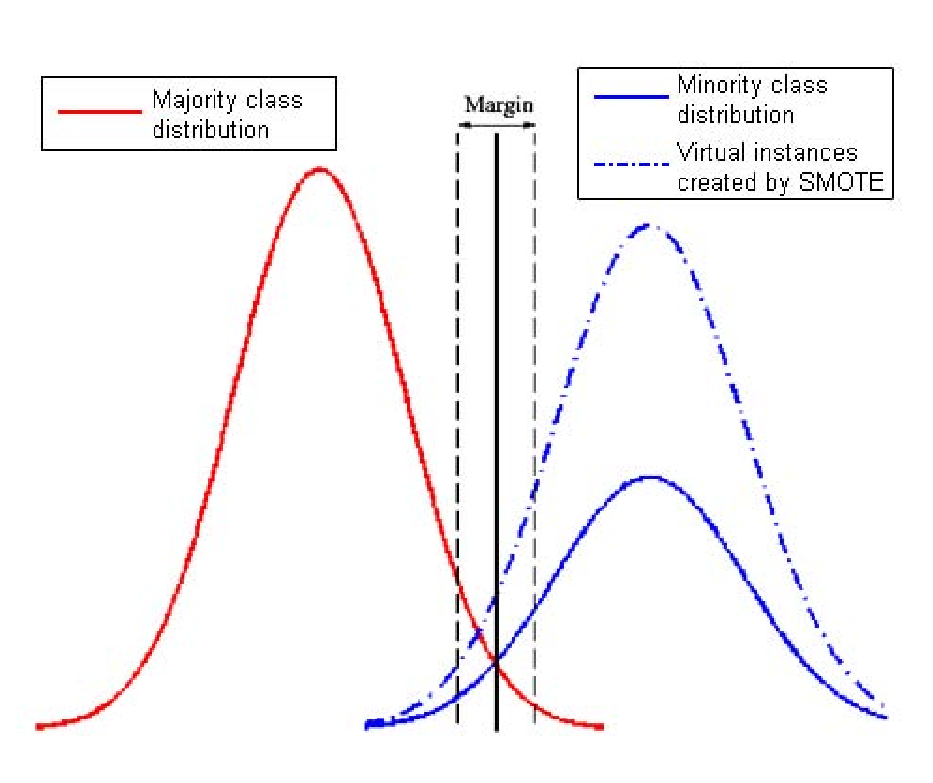
\includegraphics[width=0.45\textwidth, height=4.2cm]{Figures/virtual/smote_proc.eps}
      \label{fig:smote_sample}
      } \quad
      \subfigure[Oversampling with \textsc{Virtual}]{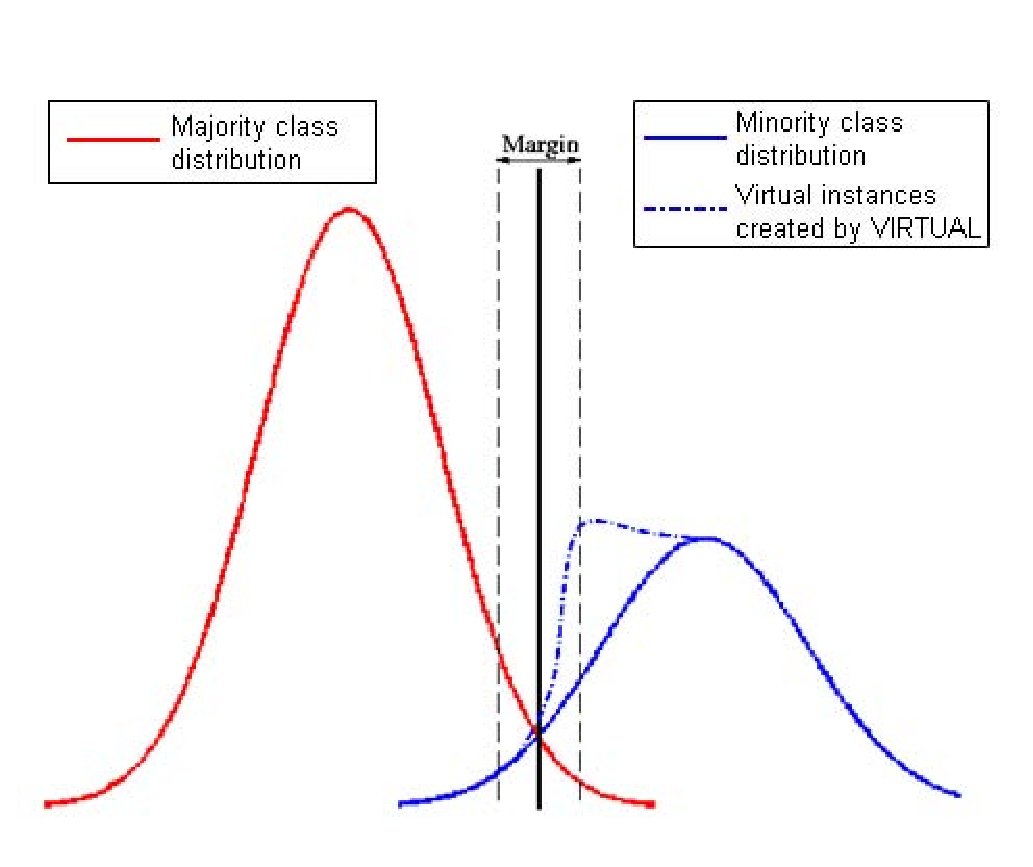
\includegraphics[width=0.45\textwidth, height=4.2cm]{Figures/virtual/virtual_proc.eps}
      \label{fig:virtual_sample}
      }
      }
    \caption{Comparison of oversampling the minority class with SMOTE and VIRTUAL. }
    \label{fig:oversample}
  \end{center}
\end{figure*}

We further analyze the computation complexity of SMOTE and \textsc{Virtual}. The computation complexity of \textsc{Virtual} is $O(\left|SV(+) \right|\cdot v \cdot \mathcal{C})$, where $v$ is the number of virtual instances created for a real positive support vector in each iteration, $\left|SV(+) \right|$ is the number of positive support vectors and $\mathcal{C}$ is the cost of finding k nearest neighbors. The computation complexity of SMOTE is $O(\left| X_R^+\right| \cdot v \cdot \mathcal{C})$, where $\left| X_R^+\right|$ is the number of positive training instances. $\mathcal{C}$ depends on the approach for finding k nearest neighbors. The naive implementation searches all $N$ training instances for the nearest neighbors and thus $\mathcal{C}=kN$. Using advanced data structure such as kd-tree, $\mathcal{C}=k\log N$. Since $\left|SV(+) \right|$ is typically much less than $\left| X_R^+\right|$, \textsc{Virtual} incurs lower computation overhead than SMOTE. Also, with fewer virtual instances created, the learner is less burdened with \textsc{Virtual}. We demonstrate with empirical results that the virtual instances created with \textsc{Virtual} are more informative and the prediction performance is also improved.

\subsection{Experiments}
We conduct a series of experiments on Reuters-21578 and four UCI datasets to demonstrate the efficacy of \textsc{Virtual}. The characteristics of the datasets are detailed in \cite{Ertekin_dissertation}. We compare \textsc{Virtual} with two systems, Active Learning (AL) and SMOTE. AL adopts the traditional active learning strategy without preprocessing or creating any virtual instances during learning. SMOTE, on the other hand, preprocesses the data by creating virtual instances before training and uses random sampling in learning. Experiments elicit the advantages of adaptive virtual sample creation in \textsc{Virtual}.

\begin{figure*}[!t]
  \centering
  \scalebox{1}
  {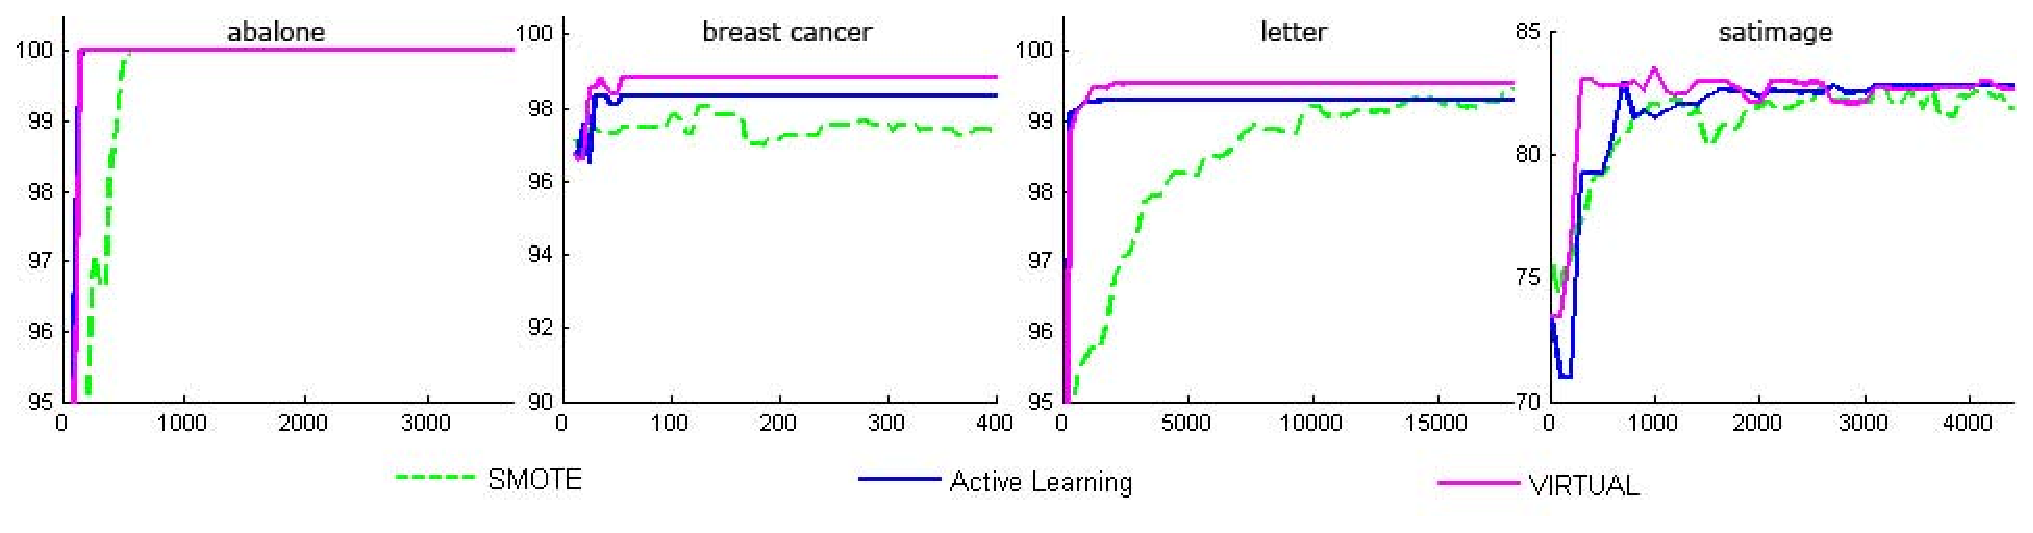
\includegraphics[width=\textwidth]{Figures/virtual/uci-graphs.eps}}\\
  \caption{Comparison of SMOTE, AL and VIRTUAL on \emph{UCI} datasets.
  We present the g-means (\%) (y-axis) of the current model for the test set
  vs. the number of training samples (x-axis) seen.}
  \label{fig:uci}
\end{figure*}


\begin{figure*}[!b]
  \centering
  \scalebox{1}
  {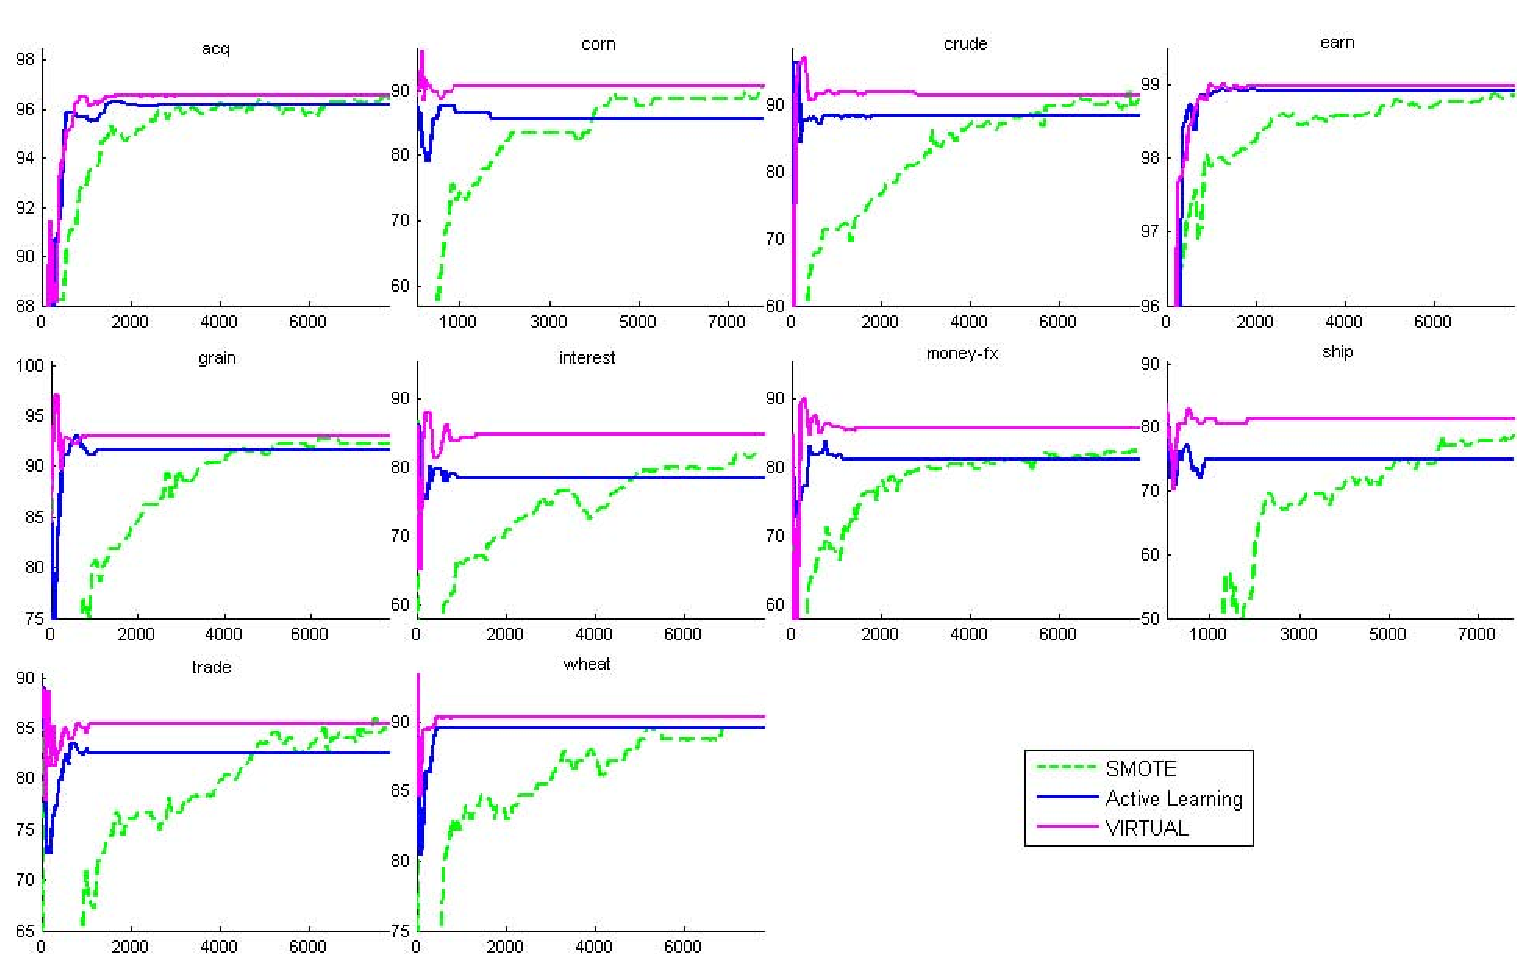
\includegraphics[width=\textwidth]{Figures/virtual/reuters.eps}}\\
  \caption{Comparison of SMOTE, AL and VIRTUAL on 10 largest categories of \emph{Reuters-21578}.
  We show the g-means (\%) (y-axis) of the current model for the test set
  versus the number of training samples (x-axis) seen.}
  \label{fig:reuters}
\end{figure*}


In Figures \ref{fig:uci} and \ref{fig:reuters} provide details on the behavior of the three algorithms, SMOTE, AL and \textsc{Virtual}. For the Reuters datasets (Figure \ref{fig:reuters}), note that in all the 10 categories \textsc{Virtual} outperforms AL in g-means metric after saturation. The difference in performance is most pronounced in the more imbalanced categories, e.g. \emph{corn}, \emph{interest} and \emph{ship}. In the less imbalanced datasets such as \emph{acq} and \emph{earn}, the difference in g-means of both methods is less noticeable. The g-means of SMOTE converges much slower than both AL and \textsc{Virtual}. However, SMOTE converges to higher g-means than AL in some of the categories, indicating that the virtual positive examples provide additional information that can be used to improve the model. \textsc{Virtual} converges to the same or even higher g-means than SMOTE while generating fewer virtual instances. For the UCI datasets (Figure \ref{fig:uci}), \textsc{Virtual} performs as well as AL in \emph{abalone} in g-means and consistently outperforms AL and SMOTE in the other three datasets.

\begin{table}[t!]
\centering \small
\caption{Support vectors with SMOTE (SMT), AL and VIRTUAL. Imb.Rt. is the data imbalance ratio and
\#SV(-)/\#SV(+) represents the support vector imbalance ratio. The rightmost two columns compare the portion of the virtual instances selected as support vectors in SMOTE and VIRTUAL.}
\small
\begin{tabular}{l@{\hspace{1mm}}|l@{\hspace{1mm}}|c@{\hspace{1mm}}|c@{\hspace{1mm}}|c@{\hspace{1mm}}|c@{\hspace{1mm}}|c@{\hspace{1mm}}|c}
\hline
\multicolumn{2}{c|}{\multirow{2}{1cm}{Dataset}}&Imb.&\multicolumn{3}{c|}{\#SV(-)/\#SV(+)}&\multicolumn{2}{c}{\#$SV_V(+)$/\#V.I.}\\\cline{4-8}
\multicolumn{2}{c|}{}&Rt.&SMT&AL&\textsc{Virtual}&SMT&\textsc{Virtual}\\
\hline\hline
\multirow{10}{2mm}{\begin{sideways}\parbox{13mm}{Reuters}\end{sideways}}
&acq&3.7&1.24&1.28&1.18&2.4\%&\textbf{20.3\%}\\
&corn&41.9&2.29&3.08&1.95&17.1\%&\textbf{36.6\%}\\
&crude&19.0&2.30&2.68&2.00&10.8\%&\textbf{50.4\%}\\
&earn&1.7&1.68&1.89&1.67&6.0\%&\textbf{24.2\%}\\
&grain&16.9&2.62&3.06&2.32&7.2\%&\textbf{42.3\%}\\
&interest&21.4&1.84&2.16&1.66&13.3\%&\textbf{72.2\%}\\
&money-fx&13.4&1.86&2.17&1.34&8.2\%&\textbf{31.1\%}\\
&ship&38.4&3.45&4.48&2.80&20.0\%&\textbf{66.5\%}\\
&trade&20.1&1.89&2.26&1.72&15.4\%&\textbf{26.6\%}\\
&wheat&35.7&2.55&3.43&2.22&12.3\%&\textbf{63.9\%}\\
\hline\hline
\multirow{4}{2mm}{\begin{sideways}\parbox{5mm}{UCI}\end{sideways}}
&abalone&9.7&0.99&1.24&0.99&30.4\%&\textbf{69.2\%}\\
&breast&1.9&1.23&0.60&0.64&2.9\%&\textbf{39.5\%}\\
&letter&24.4&1.21&1.48&0.97&0.98\%&\textbf{74.4\%}\\
&satimage&9.7&1.31&1.93&0.92&37.3\%&\textbf{53.8\%}\\
\hline
\end{tabular}
\label{tbl:res_svs}
\end{table}

In Table \ref{tbl:res_svs}, the support vector imbalance ratio of all the three methods are lower than the data imbalance ratio, and \textsc{Virtual} achieves the most balanced ratios of positive and negative support vectors in the Reuters datasets. Despite that the datasets used have different data distributions, the portion of virtual instances which become support vectors in \textsc{Virtual} consistently and significantly higher than that in SMOTE. These results confirm the previous discussion that \textsc{Virtual} is more effective in generating informative virtual instances.

Table \ref{tbl:res_all} presents g-means and the total learning time for SMOTE, AL and  \textsc{Virtual}. Classical batch SVM's g-means values are also provided as a reference point. In Reuters datasets, \textsc{Virtual} yields the highest g-means in all categories. Table 4 shows the effectiveness of adaptive virtual instance generation. In categories \emph{corn}, \emph{interest} and \emph{ship} with high class imbalance ratio, \textsc{Virtual} gains substantial improvement in g-means. Compared to AL, \textsc{Virtual} requires additional time for the creation of virtual instances and selection of those which may become support vectors. Despite this overhead, \textsc{Virtual}'s training times are comparable with that of AL. In the cases where minority examples are abundant, SMOTE demands substantially longer time to create virtual instances than \textsc{Virtual}. But as the rightmost columns in Table 3 show, only a small fraction of the virtual instances created by SMOTE become support vectors. Therefore SMOTE spends much time to create virtual instances that will not be used in the model. On the other hand, \textsc{Virtual} has already a short training time and uses this time to create more informative virtual instances. In Table 4, the numbers in parentheses give the ranks of the g-means prediction performance of the four approaches. The values in bold correspond to a win and \textsc{Virtual} wins in nearly all datasets.  The Wilcoxon signed-rank test (2-tailed) between \textsc{Virtual} and its nearest competitor SMOTE reveals that the zero median hypothesis can be rejected at the significance level 1\% ($p=4.82 \times 10^{-4}$), implying that \textsc{Virtual} performs statistically better than SMOTE in these 14 datasets. These results demonstrate the importance of creating synthetic samples from the informative examples rather than all the examples.


\begin{table*}[!tp]\centering \small
\caption{g-means and total learning time using SMOTE, AL and VIRTUAL.
`Batch' corresponds to the classical SVM learning in batch setting without resampling.
The numbers in brackets denote the rank of the corresponding method in the dataset.}
\begin{tabular}{l|l|c@{\hspace{1mm}}|c@{\hspace{1mm}}|c@{\hspace{1mm}}|c@{\hspace{1mm}}|c|r|c}
\hline
\multicolumn{2}{c|}{\multirow{2}{1cm}{Dataset}}&\multicolumn{4}{c|}{g-means (\%)}&\multicolumn{3}{c}{Total learning time (sec.)}\\\cline{3-9}
\multicolumn{2}{c|}{}&Batch&SMOTE&AL&\textsc{Virtual}&SMOTE&AL&\textsc{Virtual}\\
\hline\hline
\multirow{10}{3mm}{\begin{sideways}\parbox{13mm}{Reuters}\end{sideways}}
&acq&96.19 (3)&96.21 (2)&96.19 (3)&\textbf{96.54 (1)}&2271&146&203\\
&corn&85.55 (4)&89.62 (2)&86.59 (3)&\textbf{90.60 (1)}&74&43&66\\
&crude&88.34 (4)&91.21 (2)&88.35 (3)&\textbf{91.74 (1)}&238&113&129\\
&earn&98.92 (3)&\textbf{98.97 (1)}&98.92 (3)&\textbf{98.97 (1)}&4082&121&163\\
&grain&91.56 (4)&92.29 (2)&91.56 (4)&\textbf{93.00 (1)}&296&134&143\\
&interest&78.45 (4)&83.96 (2)&78.45 (4)&\textbf{84.75 (1)}&192&153&178\\
&money-fx&81.43 (3)&83.70 (2)&81.08 (4)&\textbf{85.61 (1)}&363&93&116\\
&ship&75.66 (3)&78.55 (2)&74.92 (4)&\textbf{81.34 (1)}&88&75&76\\
&trade&82.52 (3)&84.52 (2)&82.52 (3)&\textbf{85.48 (1)}&292&72&131\\
&wheat&89.54 (3)&89.50 (4)&89.55 (2)&\textbf{90.27 (1)}&64&29&48\\
\hline\hline
\multirow{4}{2mm}{\begin{sideways}\parbox{5mm}{UCI}\end{sideways}}
&abalone&\textbf{100 (1)}&\textbf{100 (1)}&\textbf{100 (1)}&\textbf{100 (1)}&18&4&6\\
&breast&98.33 (2)&97.52 (4)&98.33 (2)&\textbf{98.84 (1)}&4&1&1\\
&letter&99.28 (3)&99.42 (2)&99.28 (3)&\textbf{99.54 (1)}&83&5&6\\
&satimage&\textbf{83.57 (1)}&82.61 (4)&82.76 (3)&82.92 (2)&219&18&17\\
\hline
\end{tabular}
\vspace{-3mm}
\label{tbl:res_all}
\end{table*}

\drop{
\section{Conclusions}
The class imbalance problem has been known to hinder the generalization performance of classification algorithms. This chapter offers a better understanding of how active learning can remedy the problems that stem from class imbalance and presents techniques to improve the efficiency of active learning when dealing with such problems.

This chapter begins by  first present an efficient active learning method which selects informative instances from a randomly picked small pool of examples rather than making a full search in the entire training set. This strategy renders active learning to be applicable to very large datasets which otherwise would be computationally very expensive. Combined with the early stopping heuristics, active learning achieves a fast and scalable solution without sacrificing prediction performance. We then show that this active learning strategy can be used to address the class imbalance problem. In simulation studies, we demonstrate that as the imbalance ratio increases, active learning can achieve better prediction performance than random sampling by only using the informative portion of the training set. By focusing the learning on the instances around the classification boundary, more balanced class distributions can be provided to the learner in the earlier steps of the learning.  Our empirical results on a variety of real-world datasets allow us to conclude that active learning is comparable or even better than other popular resampling methods in dealing with imbalanced data classification.

The second part presents an active learning based adaptive resampling strategy, \textsc{Virtual} to address the imbalanced data classification problem in SVMs. \textsc{Virtual} adaptively creates instances according to the real positive support vectors selected in each active learning step. These instances are informative as they are close to the hyperplane. Thus \textsc{Virtual} creates fewer virtual instances that are informative. Our complexity analysis shows that \textsc{Virtual} incurs lower overhead in data generation and eventually less burden to the learner. Our thorough empirical results on both artificial and real-world data demonstrate that \textsc{Virtual} is capable of
achieving higher g-means than active learning without oversampling (AL) and SMOTE. Experimental results also show that \textsc{Virtual} is more resilient to high class imbalance ratios due to its capability of creating more balanced models using the virtual instances created. The training time of \textsc{Virtual} is substantially shorter than SMOTE in most cases.
}
